\section{Tomcat : conteneur de servlet Java EE}
%Nicolas
\subsection{Presentation}
\frame{\frametitle{Présentation Tomcat}
  \begin{itemize}
    \item Projet open-source de la fondation Apache
    \item Serveur d'applications Java
    \begin{itemize}
      \item Servlet (génération de page Html, xml etc...)
      \item JavaServer Pages
    \end{itemize}
    \item 
  \end{itemize}
  }
\frame{\frametitle{Présentation Tomcat}
		\framesubtitle{Serveur d'application}
  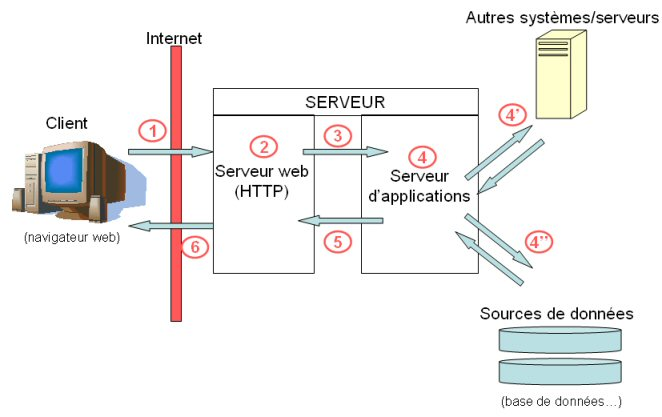
\includegraphics[scale=0.5]{Images/serveurapp.png}
}

\frame{\frametitle{Configuration Tomcat}

		\framesubtitle{Arborescence}
		Répertoire d'installation : CATALINA\_HOME
\begin{itemize} 
    \item \textbf{bin/} exécutables de Tomcat(démarrage du serveur)
    \item \textbf{common/} classes et librairies partagées par les applications web
    \item \textbf{conf/}
    \item \textbf{Logs/}
    \item \textbf{server/} contient les applications web du serveur en lui-même
    \item \textbf{shared/} contient les classes et librairies partagées par toutes les applications web hébergées sur le serveur
    \item \textbf{temp/}
    \item \textbf{webapps/} contient les applications web
    \item \textbf{work/} contient les JSP compilées
\end{itemize} 
}


\subsection{Lists I}
\frame[containsverbatim]{\frametitle{Configuration Tomcat}
\framesubtitle{Server.xml}
\begin{itemize}
\item \$CATALINA\_HOME/server.xml : principal fichier de configuration

\item Eléments conteneurs (obligatoirs) : Engine, Host, Connector
 
\item Définition des services, protocoles, port utilisés, redirection vers des ressources externes, des serveurs externes

\item Eléments facultatifs : GlobalNamingResources, Resources, Realm et Valve.


\end{itemize} 

\begin{lstlisting}
<Server port="8005" shutdown="SHUTDOWN">
...
</Server>

		\end{lstlisting}
		
}


\frame[containsverbatim]{\frametitle{Configuration Tomcat}
		\framesubtitle{Server.xml}
		Eléments Connecteur
		\begin{itemize} 
   		\item objet Java capable d'écouter un port précis et comprenant un protocole précis
    	\item redirige les requêtes qu'il reçoit au moteur de servlets du service
		\end{itemize}

		\begin{lstlisting}
<Connector port="8080"
	protocol="HTTP/1.1"
	connectionTimeout="20000"
	maxThread="100"
	maxCount="100"
	redirectPort="8443" />
		\end{lstlisting}
}



\frame[containsverbatim]{\frametitle{Configuration Tomcat}
		\framesubtitle{Server.xml}
		Eléments Engine et Host
		\begin{itemize} 
   		\item \textbf{Elément Engine} : modélise le moteur de servlet, contient un ou plusieurs
hosts
    	\item \textbf{Elément Host} hôte virtuel (doit être associé à l'adresse IP de cen serveur)
		\end{itemize}

		\begin{lstlisting}
<Engine name="Catalina">
<Host name="localhost" appBase="webapps"
unpackWARs="true" autoDeploy="true">
<!-- contenu de l'élément Host -->
</Host>
</Engine>
		\end{lstlisting}
}

\frame[containsverbatim]{\frametitle{Configuration Tomcat}
		\framesubtitle{Server.xml}
		Resssources et variables d'environnement

		\begin{lstlisting}
<GlobalNamingResources>
<Resource name="UserDatabase" auth="Container" type="org.apache.catalina.UserDatabase" description="User database that can be updated and saved" factory="org.apache.catalina.users.MemoryUserDatabaseFactory" pathname="conf/tomcat-users.xml" />
<Environment name="maxRetry" type="java.lang.Integer" value="10" override="false"/>
</GlobalNamingResources>

		\end{lstlisting}
}


\frame{\frametitle{Déploiement d'une application Tomcat}
	Installation d'une application web sous la forme d'une archive war
  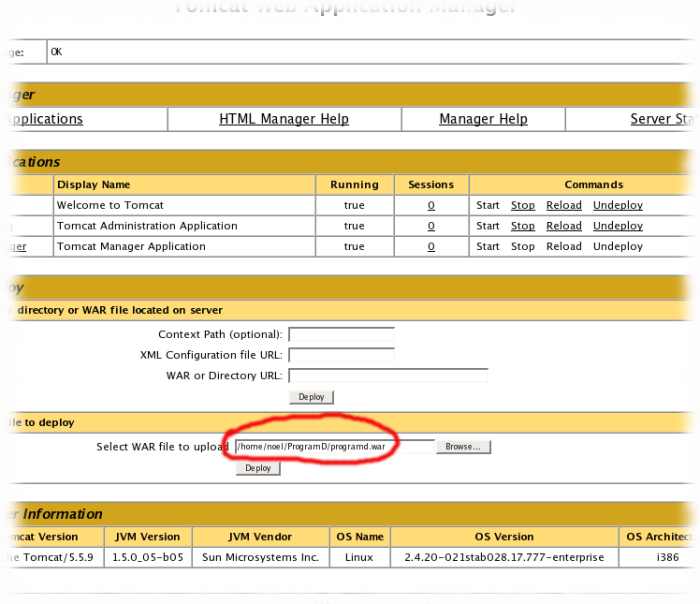
\includegraphics[scale=0.3]{Images/tomcat-deploy-war.png}
}

\frame[containsverbatim]{\frametitle{Autres serveurs d'applications existants}
En réalité, Tomcat est juste un conteneur de servlets, il existe des serveurs implémentant les normes JEE (sécurité, ejbs, transactions globales...) :
\begin{itemize} 
   		\item GlassFish
    	\item jBoss
    	\item websphere
		\end{itemize}
}

